
\section{CRIL: Compact Representation for Incremental Learning}
\label{sec:cril}

\subsection{Motivation}
\label{sec:motivation}

An exampler set is a direct factor in labeling new data as it arrives. Reducing size of exampler set is inevitable because class is added within limited budget. Therefore, it is important to ensure that the quality of the exampler set is well preserved when performing class-incremental learning.

iCaRL uses naive linear classifier to train the network to generate the output feature vecors to be linearly separable. iCaRL uses a way to sort the exampler set and to remove the worst at the reduce step so that the average feature vector can be preserved as best as possible.

\begin{figure}[h]
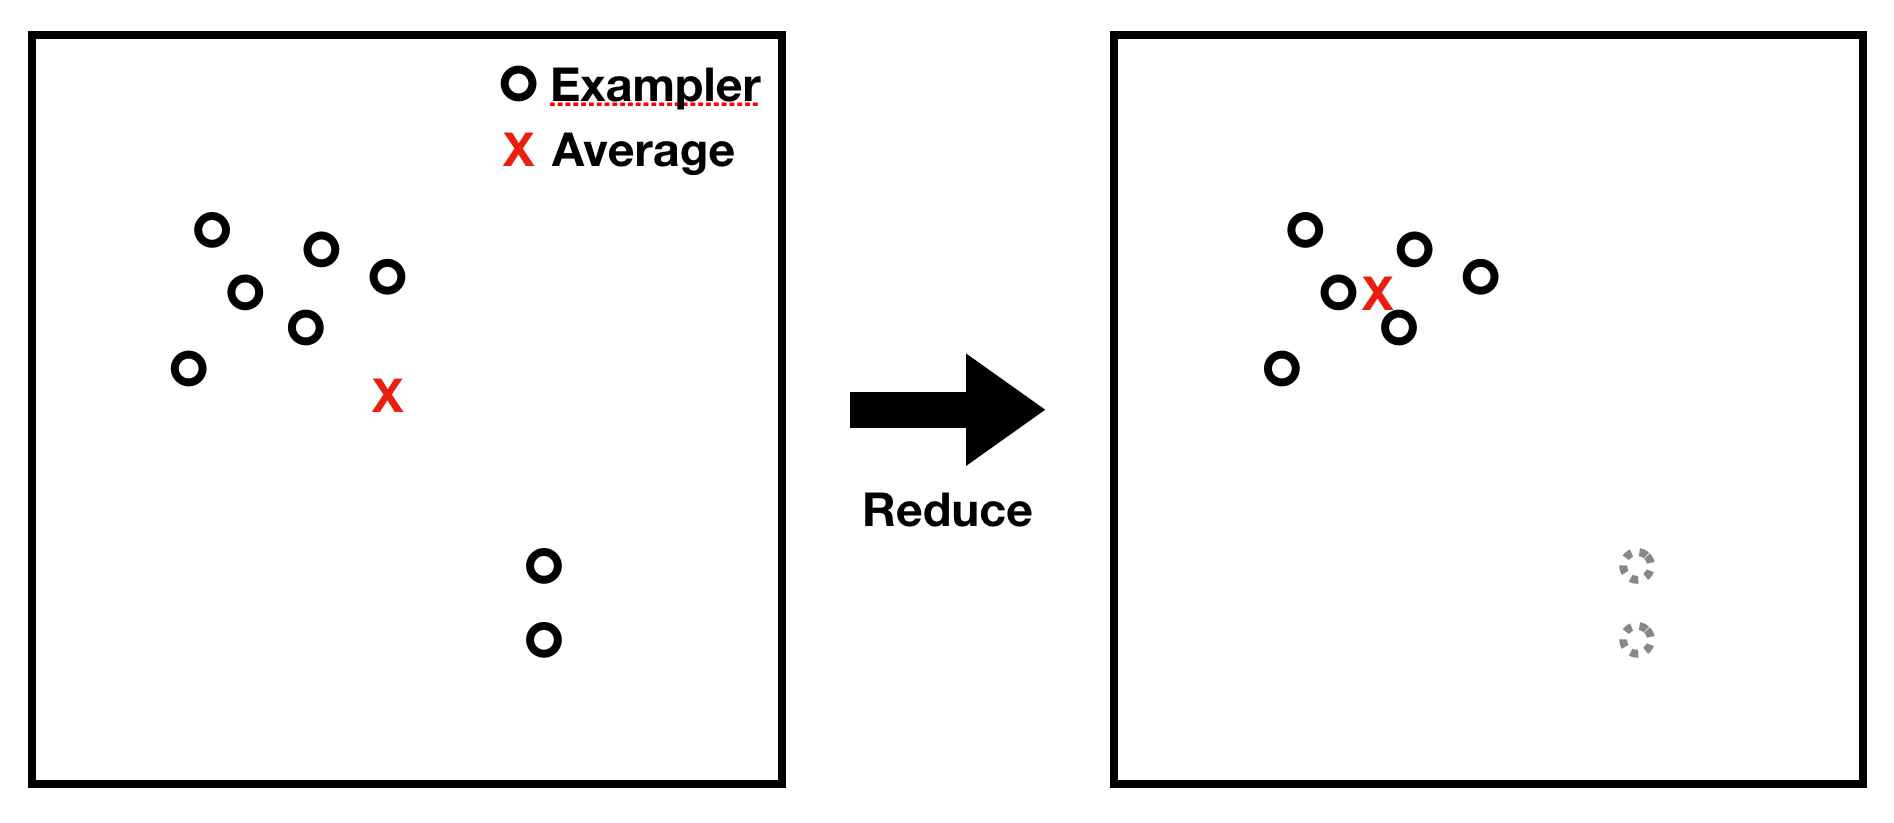
\includegraphics[width=80mm]{data/compact_motivation.png}
\centering
\caption{Change of the average feature representation. As the exampler size being reduced, the average feature representation may change its position with huge difference. \label{fig:compact_motivation}}
\end{figure}
Although the average feature vector of the initial examplers of one class may reflect the entire class well, as the size of the exampler set reduces, it can happen that the remaining examplers do not reflect the features of the class.

\subsection{CRIL}

\begin{figure}[h]
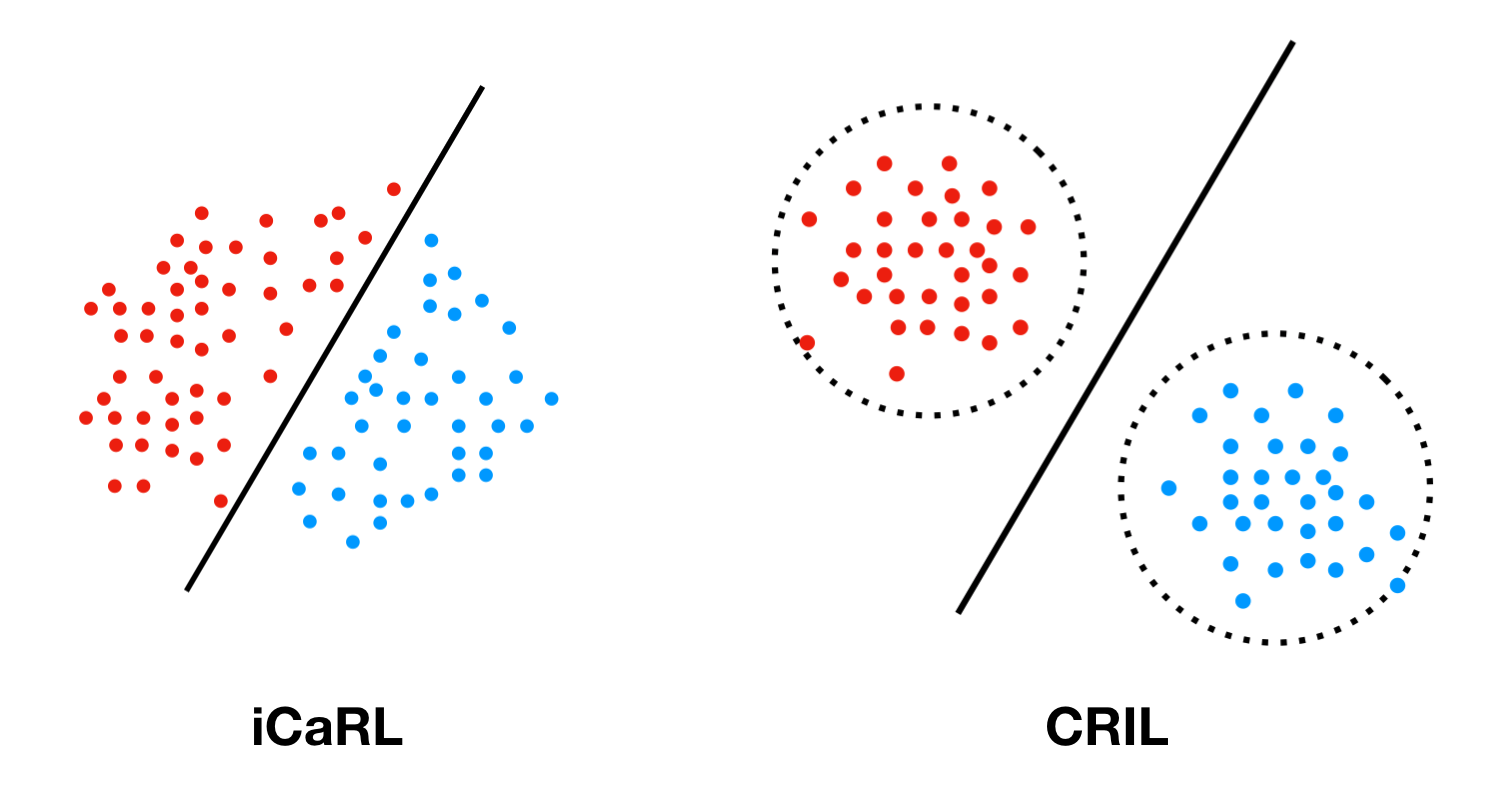
\includegraphics[width=80mm]{data/compact_representation.png}
\centering
\caption{The feature representation learning strategy for each of iCaRL and CRIL. iCaRL uses naive linear classification while CRIL applies VAE. \label{fig:compact_representation}}
\end{figure}

To solve aforementioned issue, we presents compact representation for incremental learning, CRIL.

The main idea of CRIL operates on the representation learning step. Rather than using naive linear classifier on the training to generate the output feature vectors to be linearly separable, CRIL applies variational auto encoder(VAE)~\cite{Kingma:2013aa} so that the network is trained to generate the output feature vectors following the distinctive gaussian distribution for each of the observed class. Deliberately pulling the output feature vectors between each class with a small amount of the gaussian distribution will prevent the decline of the classification competence of reduced exampler set.

The essential component for CRIL is the encoder that is going to be used as a feature extractor. Rather than use a simple network as a supervised feature extractor, we claim that the autoencoder which trains both the feature extracting model and the data generating model is more suitable method.

\subsection{Algorithm} % OR Structure OR Architecture
\label{sec:algorithm}
\todo{YOUNGKI PLEASE HELP}
